\documentclass{beamer}

\usepackage{graphicx}
\usepackage[normalem]{ulem}

\usetheme{Warsaw}
\useoutertheme{infolines}

\title{AUF/UWRA Referee Course}
\subtitle{Level 1}
\author{Carlos Ledezma}
\date{20/01/2018}

\AtBeginSection[]
{
	\begin{frame}{Outline}
		\tableofcontents[currentsection,hideothersubsections]
	\end{frame}
}

\AtBeginSubsection[]
{
	\begin{frame}{Outline}
		\tableofcontents[currentsection,currentsubsection,subsectionstyle=show/shaded/hide]
	\end{frame}
}

\begin{document}
	\begin{frame}
		\titlepage
	\end{frame}

	\begin{frame}{Outline}
		\tableofcontents[pausesections,hideallsubsections]
	\end{frame}

	\section{Introduction}
	\subsection{Motivation}

	\begin{frame}{Benefits of becoming a referee}
		What's in it for you? \pause
		\begin{itemize}
			\item Better understanding of the game \pause
			\item Better understanding as a player \pause
			\item Opportunities to travel \pause
			\item Bragging rights
		\end{itemize}
	\end{frame}

	\begin{frame}{Main responsibilities of a referee}
		\pause
		Referees guarantee:
		\begin{itemize}
			\item Fair match \pause
			\item Safe match
		\end{itemize}

		\pause

		This requires:
		\begin{itemize}
			\item Knowledge and understanding of the rules

			\pause

			\item \textbf{Impartiality}
			\item \textbf{Calmness}
		\end{itemize}
	\end{frame}

	\subsection{Structure of the course}
	\begin{frame}{Course structure}
		\begin{itemize}
			\item Theory session \pause
			\item Practical session \pause	
			\item Multiple choice exam
		\end{itemize}
	\end{frame}

	\subsection{Dynamics of the course}
	\begin{frame}{The intention}
		You are encouraged to
		\begin{itemize}
			\item Ask questions
			\item Discuss
			\item Question me $\leftarrow$
			\item Debate
		\end{itemize}

		\pause

		\begin{center}
			\textbf{\uppercase{Let's begin!}}
		\end{center}
	\end{frame}

	\section{Role of the referees}
	
	\subsection{Qualities and expectations}

	\begin{frame}{What makes a good referee?}
		\pause
		\begin{center}
			Control the game?
		\end{center}
	\end{frame}
		
	\begin{frame}{What makes a good referee?}
		\begin{center}
			\sout{Control the game?} $\rightarrow$ Game in control
		\end{center}
		\pause
		In order to keep the game in control:
		\begin{itemize}
			\item Concentration \pause $\leftarrow$ \textbf{Eyes on the game} \pause
			\item Knowing the rules \pause
			\item Positioning \pause
			\item Fitness \pause
			\item Communication \pause
			\item Composure
		\end{itemize}
	\end{frame}

	\begin{frame}{What makes a good referee?}
		Expectations: \pause
		\begin{itemize}
			\item Fairness/Safety \pause
			\item Calmness \pause
			\item Decisiveness \pause
			\item Neutrality (both in and out of the water) \pause
			\item Keep the game flowing \pause
			\item Efficiency
		\end{itemize}
	\end{frame}

	\begin{frame}{The most important rule}
		\pause
		(3.1.1) ``\textit{At least three referees shall be responsible for each match and their \textbf{decisions are 
binding.}}''

		\pause

		\begin{center}
			\textbf{\uppercase{You are in control}}
		\end{center}
	\end{frame}

	\subsection{Water referee}
	\begin{frame}{Your responsibilities}
		\begin{center}
			Observing any infringement of the rules

			Signal when a goal is scored
		\end{center}
	\end{frame}

	\begin{frame}{A matter of perspective}
		\begin{center}
			Two videos to prove a point $\leftarrow$ Referee perspective
		\end{center}
	\end{frame}

	\begin{frame}{A matter of perspective}
		\begin{tabular}{ll}
			\parbox{0.5\linewidth}{
				The first video
				\begin{itemize}
					\item Very far away
					\item Hard to see where the ball is
					\item Hard to see fouls
					\item Hard to determine goals
				\end{itemize}
				\pause
			}
			&
			\parbox{0.5\linewidth}{
				The second video
				\begin{itemize}
					\item Easy to keep track of the ball
					\item Clear view of the basket
					\item Close enough to the action
					\item Does not interfere with play
				\end{itemize}
			}
		\end{tabular}
		\pause
		\begin{center}
			\textbf{Positioning is very important}
		\end{center}
	\end{frame}

	\begin{frame}{Positioning - Transition game}
		\begin{center}
			Tendency of the game $\rightarrow$ Center of the pool
		\end{center}
	\end{frame}

	\begin{frame}{Positioning - Transition game}
		Key points:
		\begin{itemize}
			\item Be in line with the ball
			\item Stay close to the edges
			\item Avoid contact $\leftarrow$ Vertical movement
			\item Always keep sight of play
		\end{itemize}
	\end{frame}

	\begin{frame}{Positioning - Attack on goal}
		Key points:
		\begin{itemize}
			\item Always keep sight of the goal
			\item Watch for fouls under the goal
			\begin{itemize}
				\item Attacker on defender
				\item Defender on attacker
			\end{itemize}
			\item Do not interfere
		\end{itemize}
	\end{frame}

	\begin{frame}{Positioning - Attack on goal}
		Special considerations:
		\begin{itemize}
			\item Watch for exchange lane
			\item Don't get close to the goal
		\end{itemize}
	\end{frame}

	\begin{frame}{Calling fouls}
		\begin{center}
			Always make the calls \\
			(even if late)
		\end{center}
	\end{frame}

	\begin{frame}{Calling fouls}
		\begin{center}
		You stop the game \pause $\rightarrow$ Players continue \\
		What do you do? \\

		\pause

		\textbf{You stop the game}
		\end{center}
	\end{frame}

	\begin{frame}{After play stops}
		\begin{tabular}{ll}
			\parbox{0.5\linewidth}
			{
				If you stopped the match:
				\begin{enumerate}
					\item Signal the foul
					\item \textbf{Signal the free throw}
					\item Wait for restart
				\end{enumerate}

				\pause
			}
			&
			\parbox{0.5\linewidth}
			{
				If you didn't stop the match:
				\begin{enumerate}
					\item Point to the surface
					\item Mimic free throw
				\end{enumerate}
			}
		\end{tabular}
	\end{frame}

	\subsection{Surface referee}

	\begin{frame}{The common view}
		\begin{center}
		The surface referee has a less relevant role \pause

		\textbf{Big mistake}
		\end{center}
	\end{frame}

	\begin{frame}{Watching for substitutions}
		Players must:
		\begin{itemize}
			\item Enter at the appropriate time
			\item Enter at the appropriate location
			\item Change one-for-one
		\end{itemize}

		\pause

		\textbf{Especially when close to basket}
	\end{frame}

	\begin{frame}{Watching for player count}
		Counting players in the water is \textbf{hard}
		\begin{itemize}
			\item Players are constantly diving
			\item There may be time penalties

			\pause

			\item Count the bench instead.
		\end{itemize}
	\end{frame}

	\begin{frame}{Penalizations}
		\begin{tabular}{rcl}
			\parbox{0.45\textwidth}
			{
				Jumping in early \\
				Jumping in front of lane \\
				Having too many in the water
			}
			&
			$\rightarrow$
			&
			2-minute penalty
		\end{tabular}
	\end{frame}

	\begin{frame}{Starting the game}
		\begin{center}
			Deck referee \textbf{always} restarts the game
		\end{center}
	\end{frame}

	\begin{frame}{Starting the game - Free throws}
		\begin{center}
			What would you do if game starts early? \pause

			\textbf{Stop and turnover}
		\end{center}
	\end{frame}

	\begin{frame}{Starting game - Free throws}
		How to prevent false starts?
		\begin{enumerate}
			\item Wait for ball on surface
			\item Signal start
		\end{enumerate}

		\pause

		If game begins $\rightarrow$ \textbf{Stop and turnover}
	\end{frame}

	\begin{frame}{Starting the game}
		Overall considerations:
		\begin{itemize}
			\item Allow both teams to be ready
			\item Don't be pushed by players
			\item \textbf{Allow referees to be ready}
		\end{itemize}
	\end{frame}

	\begin{frame}{Safety in surface}
		When play comes to surface:
		\begin{enumerate}
			\item Watch for swim-overs
			\item Close to wall $\rightarrow$ break hussles early
		\end{enumerate}
	\end{frame}

	\subsection{Keeping control of a match}

	\begin{frame}{Definition}
		When is a match out of control?

		\pause

		\begin{itemize}
			\item Aggressive
			\item Dirty
			\item Unbalanced $\leftarrow$ Not due to skills
		\end{itemize}
	\end{frame}

	\begin{frame}{Referee attitude}
		The referees are \textbf{responsible} for the match

		When players complain:
		\begin{itemize}
			\item Players opinions are biased
			\item Don't be intimidated
			\item Be skeptical
			\item If unsure, \textbf{ask}
		\end{itemize}
	\end{frame}

	\begin{frame}{Calling fouls}
		\begin{center}
			Balance
		\end{center}
		\begin{tabular}{ll}
			\parbox{0.5\textwidth}
			{
				\begin{center}
					Safety
				\end{center}
				\begin{itemize}
					\item Is there a hazard for players?
					\item Does this merit 2-minute penalty?
					\item Is this a repeated behaviour?
				\end{itemize}
			}
			&
			\parbox{0.5\textwidth}
			{
				\begin{center}
					Fluidity
				\end{center}
				\begin{itemize}
					\item Does the carrier have advantage?
					\item Was the foul minor?
					\item Did the foul look unintentional?
				\end{itemize}
			}
		\end{tabular}
	\end{frame}

	\begin{frame}{Calling fouls}
		\begin{center}
			Reminder \\
			Play is stopped $\rightarrow$ All is invalidated
		\end{center}
	\end{frame}

	\begin{frame}{Escalation mechanisms}
		\begin{center}
			Why are they needed?
		\end{center}
	\end{frame}

	\begin{frame}{Warnings}
		\begin{center}
			Used for repeated behaviour

			They \textbf{do not} accumulate

			Can be awarded to the team
		\end{center}
	\end{frame}

	\begin{frame}{2-minute penalty}
		Used when:
		\begin{itemize}
			\item Warned foul repeats $\leftarrow$ Including team fouls
			\item Foul was severe
		\end{itemize}
	\end{frame}

	\begin{frame}{2-minute penalty}
		Implications:
		\begin{itemize}
			\item Penalized player is out
			\item Replacement is not allowed in
			\item Team plays with one less in the water
		\end{itemize}

		\pause

		This is \textbf{harsh}. Be mindful
	\end{frame}

	\begin{frame}{2-minute penalty}
		\begin{center}
			Goal scored against + numerical disadvantage $\rightarrow$ Early dismissal

			But only 1 (the longest running)
		\end{center}
	\end{frame}

	\begin{frame}{When to escalate?}
		Always use your \textbf{best judgement} first.

		\pause

		Some example situations:
		\begin{itemize}
			\item Continuous rough play
			\item Showing contempt
			\item Ignoring calls
			\item Unsportsman behaviour
			\item Continuous questioning
		\end{itemize}
	\end{frame}

	\begin{frame}{The last two escalations}
		\begin{tabular}{ll}
			\parbox{0.5\textwidth}
			{
				\begin{center}
					2+2 penalty
				\end{center}
				\begin{itemize}
					\item 2 full time penalties
					\item Start in succession
					\item Dismissed independently
				\end{itemize}
			}
			&
			\parbox{0.5\textwidth}
			{
				\begin{center}
					Expulsion from match
				\end{center}
				\begin{itemize}
					\item Player must leave pool
					\item 5-minute penalty for team
					\item Player misses next match
				\end{itemize}
			}
		\end{tabular}
	\end{frame}

	\section{The game timing system}
	\begin{frame}
		\begin{center}
			Introduction to the game timing system and practical hands on session
		\end{center}
	\end{frame}

	\section{Some procedures during a match}
	\subsection{Hand signals}

	\begin{frame}{Why hand signals?}
		\begin{center}
			\textbf{Efficient} and \textbf{direct} communication
		\end{center}
	\end{frame}

	\begin{frame}{Basic signals}
		\begin{center}
			Goal scored

			\vspace{0.5cm}

			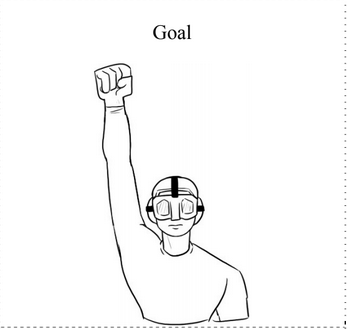
\includegraphics[scale=1.5]{goalScoredSignal}
		\end{center}
	\end{frame}

	\begin{frame}{Basic signals}
		\begin{center}
			End of period

			\vspace{0.5cm}

			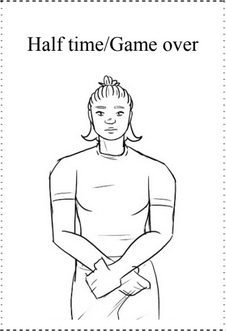
\includegraphics[scale=1.5]{endOfPeriodSignal}
		\end{center}
	\end{frame}

	\begin{frame}{Basic signals}
		\begin{center}
			Penalty shot

			\vspace{0.5cm}

			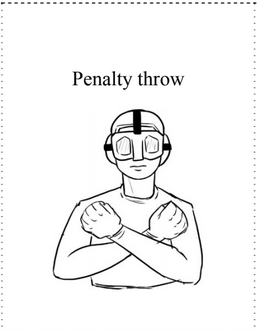
\includegraphics[scale=1.5]{penaltyShotSignal}
		\end{center}
	\end{frame}

	\begin{frame}{Basic signals}
		\begin{center}
			Holding without the ball

			\vspace{0.5cm}

			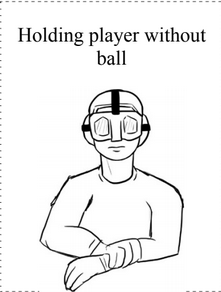
\includegraphics[scale=1.5]{holdingSignal}
		\end{center}
	\end{frame}

	\begin{frame}{Basic signals}
		\begin{center}
			Violent play

			\vspace{0.5cm}

			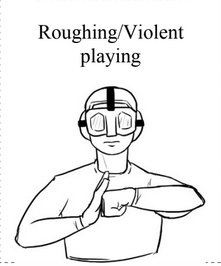
\includegraphics[scale=1.5]{violentGameSignal}
		\end{center}
	\end{frame}

	\begin{frame}{Basic signals}
		\begin{center}
			Surface referee call

			\vspace{0.5cm}

			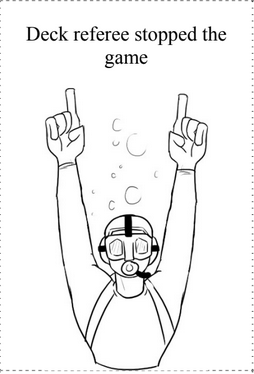
\includegraphics[scale=1.5]{surfaceRefSignal}
		\end{center}
	\end{frame}

	\begin{frame}{Basic signals}
		\begin{center}
			Water referee call

			\vspace{0.5cm}

			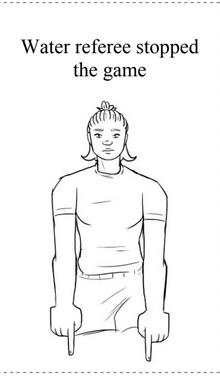
\includegraphics[scale=1.5]{waterRefSignal}
		\end{center}
	\end{frame}

	\begin{frame}{Basic signals}
		\begin{center}
			Free throw

			\vspace{0.5cm}

			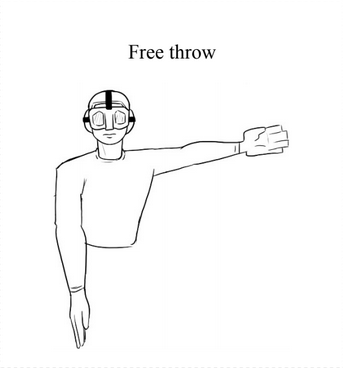
\includegraphics[scale=1.5]{freeThrowSignal}
		\end{center}
	\end{frame}

	\begin{frame}{Free throw signal}
		The most important signal:
		\begin{itemize}
			\item Used very often
			\item Indicates next action
			\item Cannot be omitted
		\end{itemize}
	\end{frame}

	\begin{frame}{Free throw signal}
		How to signal:
		\begin{itemize}
			\item Extended arm towards goal to \textbf{attack}
			\item Extended arm towards point to start

			\pause

			\item Forming an "\textbf{L}" shape \pause $\leftarrow$ You must move
		\end{itemize}
	\end{frame}

	\begin{frame}{Signal order}
		\begin{enumerate}
			\item \textbf{Stop the game}\pause
			\item Foul signal
			\item Free throw signal
			\item Wait
		\end{enumerate}

		\pause

		If you need to escalate $\rightarrow$ verbal
	\end{frame}

	\subsection{Advantage rule and delayed call}

	\begin{frame}{Definition}
		\begin{center}
			Foul happens \pause
			$\rightarrow$ \textbf{Wait} \pause
			$\rightarrow$ Call based on \textbf{advantage}
		\end{center}
	\end{frame}

	\begin{frame}{Importance}
		Why is this important? \pause

		\begin{tabular}{ll}
			\parbox{0.5\textwidth}
			{
				\begin{center}
					Prevents
				\end{center}
				\begin{itemize}
					\item Dull games
					\item Disadvantaging fouled team
					\item Players taking advantage
				\end{itemize}
			}
			\pause
			&
			\parbox{0.5\textwidth}
			{
				\begin{center}
					Guarantees
				\end{center}
				\begin{itemize}
					\item Fluidity
					\item Faster pace
					\item Fairness
				\end{itemize}
			}
		\end{tabular}
		\pause
		\begin{center}
			These will be most of your calls
		\end{center}
	\end{frame}

	\begin{frame}{Precautions}
		\begin{center}
			Never use when there is a \textbf{safety concern}
		\end{center}
	\end{frame}

	\begin{frame}{Some considerations}
		A couple things to keep in mind:
		\begin{itemize}
			\item Doesn't affect call order \pause
			\item It is \textbf{not optional} \pause
			\item Only \textbf{before} calls
		\end{itemize}
	\end{frame}

	\subsection{Penalty shots}

	\begin{frame}{Definition}
		\begin{center}
			One attacker Vs. One defender for 45 seconds
		\end{center}
	\end{frame}

	\begin{frame}{Foul penalties}
		\begin{center}
			Any foul that would prevent a goal \pause $\rightarrow$ 2-minutes
		\end{center}
	\end{frame}

	\begin{frame}{Penalty shootouts}
		\begin{tabular}{lcl}
			\parbox{0.4\textwidth}
			{
				Drawed match \\
				Requires decision
				\pause
			}
			&
			$\rightarrow$
			&
			\parbox{0.4\textwidth}
			{
				3 each (+ 1 each until decision) \\
				No repeated attackers
			}
		\end{tabular}

		\pause

		\begin{center}
			Time penalties miss first shot
		\end{center}
	\end{frame}

	\begin{frame}{Refereeing - Surface}
		\begin{tabular}{ll}
			\parbox{0.5\textwidth}
			{
				\begin{center}
					Before starting
				\end{center}
				\begin{itemize}
					\item Defender over goal
					\item Attacker in middle
					\item Referees ready
				\end{itemize}
			}
			&
			\parbox{0.5\textwidth}
			{
				\begin{center}
					During shot
				\end{center}
				\begin{itemize}
					\item Time
					\item End in the surface
				\end{itemize}
			}
		\end{tabular}
	\end{frame}

	\begin{frame}{Referreing - Water}
		\begin{center}
			\textbf{Positioning} is crucial \pause

			Keep eyes on the goal and both players
		\end{center}
	\end{frame}

	\begin{frame}{Refereeing - Water}
		Fouls around the goal
		\begin{itemize}
			\item Attack on gear
			\item Grabbing basket
			\item Goalkeeper reaching out
		\end{itemize}

		\pause

		You can play \textbf{advantage} during a penalty
	\end{frame}

	\section{Practical examples}

	\begin{frame}{Practical examples}
		\begin{center}
			\uppercase{What's the call ref?!}
		\end{center}
	\end{frame}

	\section{Conclusion}

	\begin{frame}{Before you leave}
		\pause
		\begin{itemize}
			\item Trust your judgement over the players' \pause
			\item Keep your knowledge up-to-date \pause
			\item During matches, remain calm \pause
			\item Like all of us, you are human \pause
			\item You control the tempo and fluidity. Use advantage.
		\end{itemize}

		 \pause

		\begin{center}
			\textbf{\uppercase{Get in the water!}}
		\end{center}
	\end{frame}
\end{document}
